Il modello che andremo a presentare si prefigge lo scopo di esplorare un territorio
in cui possono esserci degli ostacoli insormontabili. Si tratta di un modello distribuito; in questo modo
si può contrastare il problema del single point of failure; tuttavia per poter
sopperire a questo problema ogni robot deve possedere una certa capacità computazionale ed
una buona capacità comunicativa. Questi robot dovranno dunque essere in grado di comunicare tra loro; dovranno
inoltre essere in grado di selezionare obiettivi e percorsi; in fine dovranno avere modo di salvare la mappa.\\
Il modello è scalabile ma bisogna tenere in considerazione la quantità di dati che vengono scambiati tra i robot
all'aumentare degli stessi.
\subsection{Classificazione in quanto sistema di robot}
Secondo la tassonomia di Dudek et al \cite{dudek1996taxonomy} il nostro modello
ricade nelle categorie:
\begin{itemize}
	\item per quantità, SIZE-LIM: i robot sono pochi rispetto alla dimensione
	      dell'ambiente
	\item per raggio di comunicazione, COM-INF: ogni robot può comunicare con
	      qualsiasi altro robot.
	\item per topologia di comunicazione, TOP-BROAD: ogni messaggio è ricevuto
	      da ogni robot (broadcast)
	\item per banda di comunicazione, BAND-INF: non modelliamo il costo delle
	      comunicazioni, anche se vedremo che si ricava facilmente un limite
	      superiore
	\item per flessibilità di riposizionamento, ARR-DYN: ogni robot si muove
	      indipendentemente dai movimenti degli altri robot.
	\item per potenza elaborativa, PROC-TME: il calcolo del goal richiede una
	      macchina di turing
	\item per composizione del gruppo, COMP-IDENT: i robot sono identici tra loro	
\end{itemize}
\subsection{Ambiente}
	I robot si muovono in una griglia rettangolare. L'ambiente è:
	\begin{itemize}
		\item discreto: è diviso in celle che si classificano come
		\begin{itemize}
			\item Empty
			\item Obstacle
		\end{itemize}
		\item statico: una volta esplorata, una cella non cambia stato
		\item accessibile: il robot conosce lo stato delle celle circostanti
		\item deterministico: non c'è incertezza sullo stato del sistema
	\end{itemize}
	La griglia impedisce che due agenti si trovino stessa cella; tale scelta
	di modellazione è data dal fatto che la compresenza sarebbe inutile ai fini
	esplorativi, dato che i robot sono intercambiabili e identici.
\subsection{Interazione}
  \subsubsection{Tra agenti}
    I robot hanno un'interazione diretta attraverso una comunicazione in
    broadcast.
	Ogni robot ha conoscenza a priori dell'esistenza di tutti gli altri e invia
	un messaggio circa la sua posizione e le sue scoperte ad ogni step.
  \subsubsection{Con l'ambiente}
    I robot interagiscono con l'ambiente muovendosi in una delle celle
    dell'8-vicinato.
    Dato il modello sensoriale, lo stato della cella in cui si muoveranno è
    noto.
\subsection{Percezione}
  Ogni robot percepisce lo stato di tutte le celle comprese nel suo 8-vicinato,
  che può essere Obstacle o Empty.
  Ai fini della simulazione, lo stato viene aggornato (ovvero, i robot
  broadcastano lo stato loro circostante) alla fine di ogni turno, cioè dopo che
  tutti i robot hanno compiuto la loro mossa
\subsection{Complessità delle mappe}
\label{mapcomplex}
  Per poter caratterizzare le proprietà degli approcci da noi testati è necessario
  avere una misura che renda conto della difficoltà di esplorare una mappa.
  Le metriche esistenti affrontano il problema dal punto di vista della risoluzione
  di un labirinto con un ingresso e un'uscita. Tale approccio non si adatta al 
  nostro caso, poiché
  \begin{itemize}
	\item Tutta la mappa deve essere esplorata
	\item Non ha senso definire un ingresso e un'uscita
  \end{itemize}
  Si rende pertanto necessario trovare una metrica alternativa che sia:
  \begin{itemize}
	\item indipendente dalla dimensione della mappa: una mappa senza ostacoli 
	      deve presentare la stessa metrica qualunque sia la sua dimensione.
	\item proporzionale all'incremento di lunghezza dei percorsi causato dalla
	      morfologia della mappa.
  \end{itemize}
  Chiameremo questa misura \emph{intralcio medio}; date due celle $i$ e $j$ a 
  distanza di Chebychev $d_{ij}$, sia $p_{ij}$ il percorso minimo che le
  collega, $|p_{ij}|$ la sua lunghezza e definiamo $|p_{ij}| = +\infty$ se tale
  percorso non esiste; $k_m$ è l'intralcio medio sulla mappa m
  se in media $$|p_{ij}| = d_{ij} * k_m$$ 
  Sia $C = \{ (i,j) | i,j \in Cells, i \neq j \} $, allora
  $$k_m = \frac{1}{|C|} \sum_{(i,j) \in C}\frac{|p_{ij}|}{d_{ij}}$$
  Si deducono facilmente le seguenti proprietà:
  \begin{itemize}
	\item $\forall m, k_m \geq 1$
	\item Se m non contiene ostacoli, $k_m = 1$
    \item Se una zona non è raggiungibile in m da un'altra, $k_m = +\infty$
  \end{itemize}
  È chiaro che calcolare il percorso minimo tra ogni coppia di celle diventa
  presto dispendioso man mano che cresce la mappa, occorre quindi approssimare 
  $k_m$ con una stima $\hat{k_m}$.
  Supponiamo di calcolare, data una cella $i$,
  $$k_m^i = \frac{1}{|Cells| - 1} \sum_{j \in Cells \setminus \{i\}}\frac{|p_{ij}|}{d_{ij}}$$
  Si può mostrare che la media dei $k_m^i$ è $k_m$:
  $$k_m = \frac{1}{|Cells|}\sum_{i \in Cells} k_m^i$$
  Date le regole di movimento del nostro modello notiamo che
  \begin{itemize}
  	\item se $i$ è raggiungibile da $j$, vale anche l'inverso
    \item se quindi esiste una coppia $(a,b)$ di celle non raggiungibili tra
	      loro, presa una cella qualsiasi $i$, almeno una tra $a$ e $b$ sarà
          irraggiungibile da $i$; se ciò non fosse vero (da $i$ raggiungo sia
          $a$ che $b$), potrei costruire un percorso $a \rightarrow i
          \rightarrow b$ valido.
    \item dunque se esiste una coppia $(a,b)$ di celle non raggiungibili tra
	      loro, $\forall i, k_m^i = +\infty$.
  \end{itemize}
  Questo assicura che è sufficiente un solo $k_i$ per stabilire se $k_m = +\infty$.
  Se d'altro canto la quantità $k_m$ è finita, occorrerà calcolare più $k_m^i$ per 
  approssimarla.
  
  Dai nostri test risulta che per generare mappe di complessità arbitraria
  secondo questa metrica, un buon metodo è generare una spirale; più alto è il
  numero di spire, più alto sarà l'intralcio medio. Sebbene questa sia una 
  situazione del tutto artificiale, è interessante dal punto di vista teorico.
  \begin{figure}[H]
  \centering
  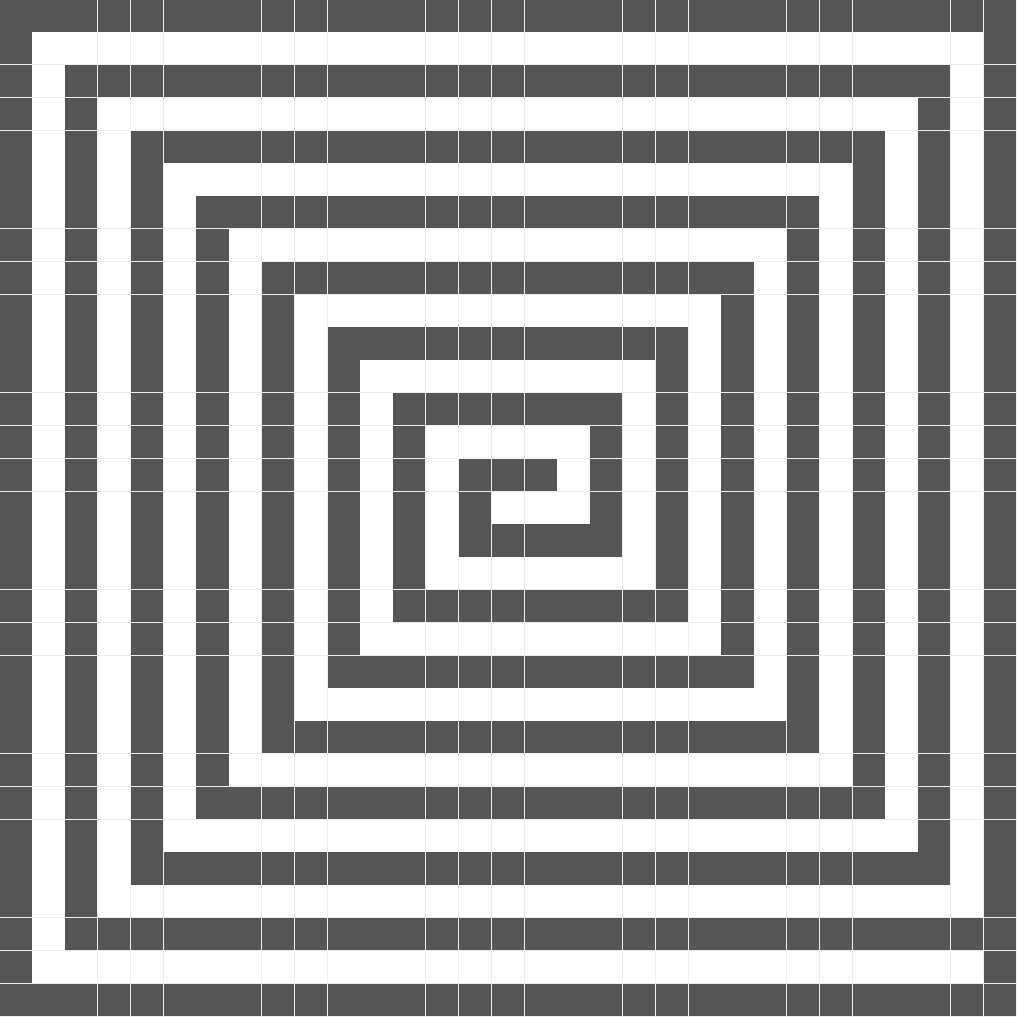
\includegraphics[width=.6\textwidth]{./immagini/mspirale.pdf}
  \caption{Una mappa a spirale con 7 avvolgimenti e intralcio medio di 12.9}
  \end{figure}
\subsection{Cattivi comportamenti}
  Su mappe che presentano una complessità elevata l'algoritmo simple può esibire
  comportamenti periodici. Facciamo qualche considerazione sul modello:
  \begin{itemize}
    \item lo stato dell'esplorazione è completamente definito dalla posizione
    degli agenti e dall'insieme delle celle, ciascuna nei 3 stati possibili per
    le celle
    \item lo stato successivo è derminato univocamente a partire dall'attuale
    \item il numero di celle è considerato finito
  \end{itemize}
  Da ciò segue che l'esplorazione può trovarsi in un numero finito di stati;
  questo ci assicura di non avere a che fare con un Halting Problem \cite{wiki:halting},
  e che anzi sicuramente, in presenza di un comportamento periodico, il sistema
  passerà più volte da uno stesso stato; ciò fornisce un metodo per poter rilevare
  con certezza tali comportamenti ciclici, seppure non di pratico utilizzo.
\subsection{Strumenti utilizzati}
  Per poter simulare e testare il modello è stato utilizzato il linguaggio
  Python unito con il framework mesa appositamente progettato per simulazioni
  multi-agente.
\subsection{Discrepanze implementative}
  A differenza di quanto descritto nel modello a livello implementativo la mappa
  è unica; tuttavia questo non modifica il comportamente descritto.
  Un'altra differenza tra modello e implementazione è il fatto che nel framework 
  i robot si muovono uno per volta mentre nel modello dovrebbero muoversi
  contemporaneamente. Tuttavia questa differenza dovrebbe essere vista come
  l'introduzione di una priorità di movimento necessaria nel caso di contese di
  una cella.
